\documentclass[11pt]{article}

% ---- Geometry & Spacing (JACMP style) ----
\usepackage[margin=1in]{geometry}
\usepackage{setspace}
\onehalfspacing
\usepackage{lineno}

% ---- Mathematics ----
\usepackage{amsmath}
\usepackage{amssymb}

% ---- Graphics & Tables ----
\usepackage{graphicx}
\usepackage{subcaption}
\usepackage{booktabs}
\usepackage{multirow}
\usepackage{array}

% ---- Colors (must precede tikz) ----
\usepackage[dvipsnames]{xcolor}

% ---- TikZ for figures ----
\usepackage{tikz}
\usetikzlibrary{arrows.meta, positioning, shapes.geometric, fit, calc, backgrounds, decorations.pathreplacing}
\usepackage{pgfplots}
\pgfplotsset{compat=1.18}

% ---- Colors & Links ----
\definecolor{pwmBlue}{HTML}{2E5FA1}
\definecolor{pwmGreen}{HTML}{3D9E3F}
\definecolor{pwmRed}{HTML}{C93C3C}
\definecolor{pwmOrange}{HTML}{E8712B}
\definecolor{pwmPurple}{HTML}{7B4EA3}
\definecolor{pwmGray}{HTML}{6B6B6B}
\usepackage[colorlinks=true, linkcolor=pwmBlue, citecolor=pwmBlue, urlcolor=pwmBlue]{hyperref}
\usepackage[capitalise,noabbrev]{cleveref}

% ---- Bibliography ----
\usepackage[numbers,sort&compress]{natbib}

% ---- Listings ----
\usepackage{listings}
\lstset{
  basicstyle=\small\ttfamily,
  breaklines=true,
  frame=single,
  xleftmargin=1em,
  framexleftmargin=0.5em,
  columns=fullflexible,
  keywordstyle=\color{pwmBlue},
  commentstyle=\color{gray},
}

% ---- Abbreviations ----
\newcommand{\pwm}{\textsc{pwm}}
\newcommand{\ie}{\textit{i.e.}}
\newcommand{\eg}{\textit{e.g.}}
\newcommand{\etc}{\textit{etc.}}
\newcommand{\etal}{\textit{et al.}}

% ===========================================================================
\title{%
  CT QC Copilot: Clinical Implementation of an\\
  Automated Quality-Control Decision-Support System}

\author{Chengshuai Yang\\
NextGen PlatformAI C Corp\\
\texttt{integrityyang@gmail.com}}

\date{February 2026}

\begin{document}
\maketitle
\linenumbers

% ===========================================================================
\begin{abstract}
We describe the clinical implementation of the CT QC Copilot, an
automated decision-support system for computed tomography quality
control.
The Copilot embodies a ``system computes, physicist decides'' model:
it automates the end-to-end QC workflow---from DICOM ingestion
through metric computation, threshold evaluation, statistical drift
detection, and root-cause diagnosis---while preserving the qualified
medical physicist's (QMP) role as the final decision-maker.
We present the clinical workflow, define the human--AI responsibility
boundary, and report results from a deployment evaluation on a
simulated 30-scanner fleet.
The Copilot reduced per-scanner QC analysis time from an estimated
$67 \pm 12$~minutes (manual) to $4.2 \pm 0.8$~minutes (automated
computation plus physicist review), a 94\% reduction that makes
AAPM TG-233 trending-based QC practical for large clinical
operations.
Western Electric rule-based drift detection identified gradual
degradation 3--6~months before threshold exceedance in 4 of 30
simulated scanners, demonstrating the early-warning value of
statistical process control.
All nine ACR-aligned metrics showed agreement with manufacturer
console values within 1.2~HU for CT number metrics and within
0.15~mm for geometric metrics.
Source code is available at
\url{https://github.com/integritynoble/Physics_World_Model}.
\end{abstract}

\noindent\textbf{Keywords:}
CT quality control, decision support, copilot model, clinical
workflow, statistical process control, AAPM TG-233

% ===========================================================================
\section{Introduction}
\label{sec:intro}

Quality control of computed tomography scanners is a foundational
responsibility of the qualified medical physicist
(QMP)~\cite{acr_ct_accreditation}.
The ACR CT Accreditation Program mandates periodic phantom-based
testing~\cite{acr_ct464}, and AAPM Task Group 233 recommends
trending-based QC with statistical process control (SPC) rather
than binary pass/fail testing~\cite{aapm_tg233}.
Despite these recommendations, the workflow at most clinical sites
remains manual: a technologist acquires phantom images, the physicist
opens vendor-specific software, manually places regions of interest,
records values in spreadsheets, and writes a summary
report~\cite{nowik2015ct_qa_automation}.

This manual process faces three scaling challenges.
First, a single QMP may oversee 10--50 CT scanners, each requiring
monthly QC with annual comprehensive
evaluations~\cite{bushberg2012essential_physics}.
At 30 scanners, manual analysis at 1--2 hours per scanner per month
amounts to 360--720 physicist-hours per year devoted to routine
computation---time diverted from clinical consultation, protocol
optimization, and radiation safety.
Second, trending-based QC requires maintaining time-series databases
and computing control-chart statistics---tasks that are error-prone
when performed in spreadsheets~\cite{pawlicki2005spc}.
Third, when metrics fail, root-cause identification requires
correlating multiple artifact signatures against known failure
modes---a cognitive task that benefits from systematic computational
support~\cite{hsieh2009computed_tomography}.

Existing solutions address parts of this problem.
Commercial QC packages (\eg, Sun Nuclear, Radcal) automate portions
of the analysis but operate as closed-source
systems~\cite{aapm_tg233}.
Open-source tools such as pydicom~\cite{pydicom} provide DICOM
handling but not integrated QC workflows.
Nowik \etal~\cite{nowik2015ct_qa_automation} demonstrated automated
phantom analysis but without SPC integration or diagnostic support.
Able \etal~\cite{able2016spc_ct} applied SPC to CT constancy testing
but did not provide a complete decision-support framework.

We present the CT QC Copilot, a decision-support system that
automates the computational aspects of CT QC while preserving the
physicist's role as the decision-maker (\cref{fig:copilot_model}).
The Copilot builds on the open-source \pwm{} CT QC
Platform~\cite{pwm_platform}, inheriting its CasePack workflow
specification, four-layer threshold system, and immutable baselines.
This paper focuses on the \emph{clinical implementation}: how the
Copilot integrates into the physicist's workflow, what decisions
it supports, and what operational impact it achieves.


% ===========================================================================
% FIGURE 1: Copilot Model -- Human-AI Responsibility Boundary
% ===========================================================================
\begin{figure}[t]
\centering
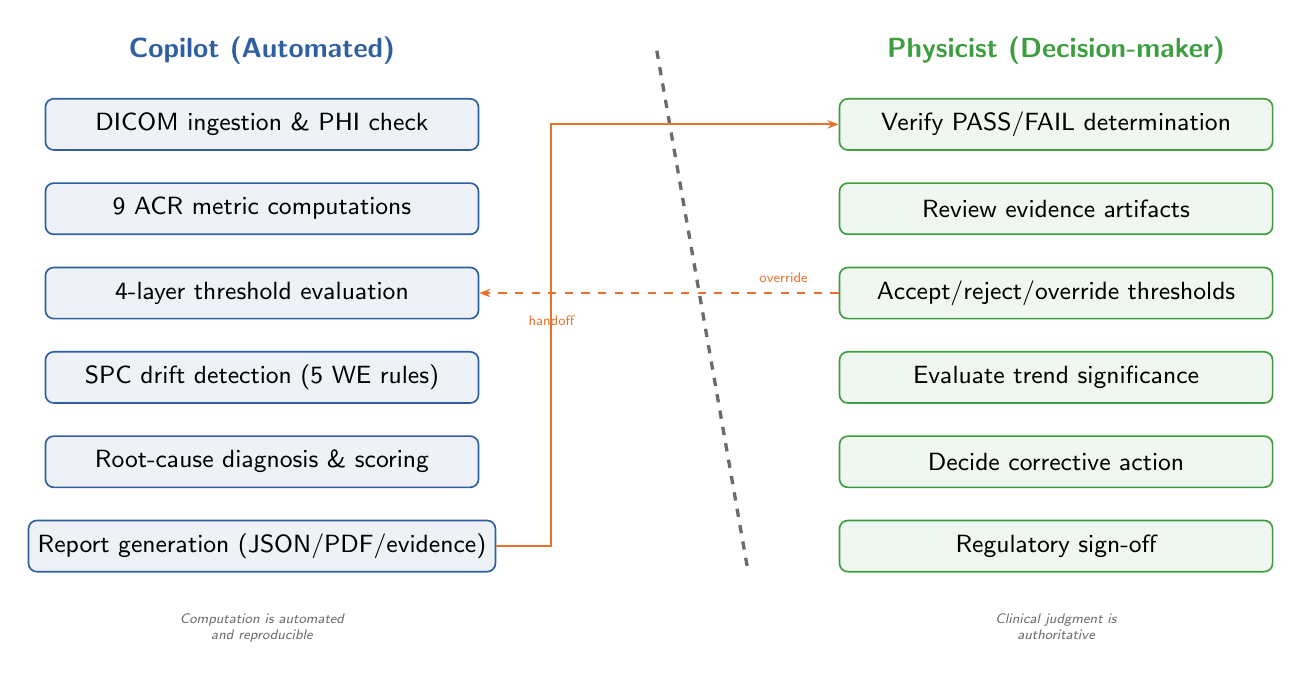
\begin{tikzpicture}[
  node distance=0.4cm,
  aibox/.style={
    rectangle, rounded corners=3pt, draw=pwmBlue, fill=pwmBlue!8,
    minimum width=5.5cm, minimum height=0.65cm,
    font=\small\sffamily, line width=0.6pt,
  },
  humanbox/.style={
    rectangle, rounded corners=3pt, draw=pwmGreen, fill=pwmGreen!8,
    minimum width=5.5cm, minimum height=0.65cm,
    font=\small\sffamily, line width=0.6pt,
  },
  divider/.style={line width=1.2pt, pwmGray},
]

% AI side
\node[font=\sffamily\bfseries\color{pwmBlue}] (ai_title) {Copilot (Automated)};
\node[aibox, below=0.3cm of ai_title] (a1) {DICOM ingestion \& PHI check};
\node[aibox, below=of a1] (a2) {9 ACR metric computations};
\node[aibox, below=of a2] (a3) {4-layer threshold evaluation};
\node[aibox, below=of a3] (a4) {SPC drift detection (5 WE rules)};
\node[aibox, below=of a4] (a5) {Root-cause diagnosis \& scoring};
\node[aibox, below=of a5] (a6) {Report generation (JSON/PDF/evidence)};

% Divider
\draw[divider, dashed] ([xshift=3.2cm]ai_title.east) -- ([xshift=3.2cm]a6.south east);

% Human side
\node[font=\sffamily\bfseries\color{pwmGreen}, right=6.0cm of ai_title] (h_title) {Physicist (Decision-maker)};
\node[humanbox, below=0.3cm of h_title] (h1) {Verify PASS/FAIL determination};
\node[humanbox, below=of h1] (h2) {Review evidence artifacts};
\node[humanbox, below=of h2] (h3) {Accept/reject/override thresholds};
\node[humanbox, below=of h3] (h4) {Evaluate trend significance};
\node[humanbox, below=of h4] (h5) {Decide corrective action};
\node[humanbox, below=of h5] (h6) {Regulatory sign-off};

% Cross-boundary arrows
\draw[-{Stealth[length=4pt]}, pwmOrange, line width=0.7pt]
  (a6.east) -- ++(0.7,0) |- (h1.west)
  node[pos=0.25, above, font=\tiny\sffamily\color{pwmOrange}] {handoff};

\draw[-{Stealth[length=4pt]}, pwmOrange, line width=0.7pt, dashed]
  (h3.west) -- ++(-0.7,0) |- (a3.east)
  node[pos=0.25, above, font=\tiny\sffamily\color{pwmOrange}] {override};

% Bottom label
\node[font=\tiny\sffamily\itshape\color{pwmGray}, below=0.4cm of a6, text width=5cm, align=center]
  {Computation is automated\\and reproducible};
\node[font=\tiny\sffamily\itshape\color{pwmGray}, below=0.4cm of h6, text width=5cm, align=center]
  {Clinical judgment is\\authoritative};

\end{tikzpicture}
\caption{%
  The copilot model: division of responsibility between the automated
  system (left) and the qualified medical physicist (right).
  Solid orange arrow: the Copilot hands off drafted reports for
  physicist review.
  Dashed orange arrow: the physicist may override threshold
  configuration, which feeds back into future evaluations.
  The boundary ensures automation enhances rather than replaces
  professional judgment.
}
\label{fig:copilot_model}
\end{figure}


% ===========================================================================
\section{The Copilot Model}
\label{sec:copilot_model}

The term ``copilot'' encodes a specific design philosophy: the
system assists but does not replace the physicist.
We define the responsibility boundary explicitly
(\cref{fig:copilot_model}):

\paragraph{The Copilot provides:}
(i)~automated metric computation with full derivation records;
(ii)~threshold evaluation against a four-layer hierarchy (standard
$\to$ scanner model $\to$ protocol $\to$ site override);
(iii)~statistical drift detection via Shewhart charts with five
Western Electric rules~\cite{shewhart1931,western_electric_1956};
(iv)~scored root-cause hypotheses when metrics fail;
(v)~triple-output reporting (JSON, PDF, evidence artifacts); and
(vi)~``what test next?'' recommendations when diagnoses are ambiguous.

\paragraph{The physicist provides:}
(i)~clinical judgment on whether computational results are
clinically significant;
(ii)~accept/reject/investigate decisions on each metric and the
overall determination;
(iii)~verification that automated results are plausible;
(iv)~corrective action decisions based on diagnostic hypotheses;
and (v)~regulatory sign-off constituting the official QC record.

This division is consistent with AAPM guidance on the role of the
QMP~\cite{aapm_tg233} and with the FDA's framework for clinical
decision-support software~\cite{samd_fda}.
The physicist may override any Copilot determination; the Copilot's
role terminates at recommendation.


% ===========================================================================
% FIGURE 2: Clinical Workflow
% ===========================================================================
\begin{figure}[t]
\centering
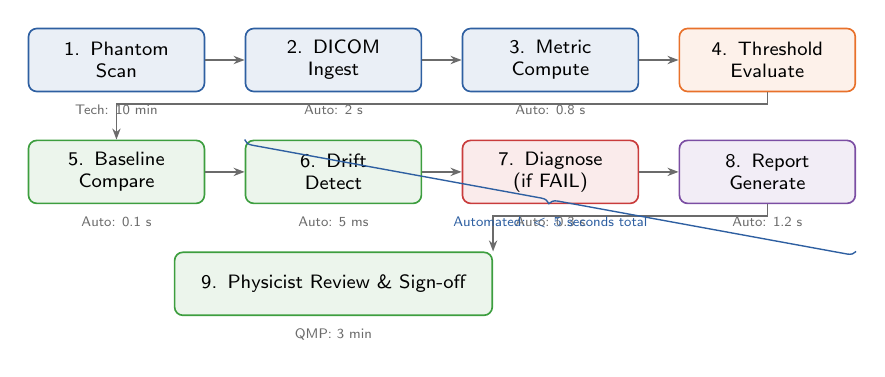
\begin{tikzpicture}[
  node distance=0.35cm and 0.5cm,
  step/.style={
    rectangle, rounded corners=3pt, draw=#1, fill=#1!10,
    minimum width=2.2cm, minimum height=0.8cm,
    font=\scriptsize\sffamily, text width=2.0cm, align=center,
    line width=0.6pt,
  },
  arrow/.style={-{Stealth[length=4pt]}, line width=0.6pt, color=pwmGray},
  timelab/.style={font=\tiny\sffamily\color{pwmGray}, below=1pt},
]

% Steps
\node[step=pwmBlue] (s1) {1. Phantom\\Scan};
\node[step=pwmBlue, right=of s1] (s2) {2. DICOM\\Ingest};
\node[step=pwmBlue, right=of s2] (s3) {3. Metric\\Compute};
\node[step=pwmOrange, right=of s3] (s4) {4. Threshold\\Evaluate};
\node[step=pwmGreen, below=0.6cm of s1] (s5) {5. Baseline\\Compare};
\node[step=pwmGreen, right=of s5] (s6) {6. Drift\\Detect};
\node[step=pwmRed, right=of s6] (s7) {7. Diagnose\\(if FAIL)};
\node[step=pwmPurple, right=of s7] (s8) {8. Report\\Generate};

% Physicist review
\node[step=pwmGreen, below=0.6cm of s6, minimum width=4.0cm, text width=3.8cm]
  (s9) {9. Physicist Review \& Sign-off};

% Arrows
\draw[arrow] (s1) -- (s2);
\draw[arrow] (s2) -- (s3);
\draw[arrow] (s3) -- (s4);
\draw[arrow] (s4.south) -- ++(0,-0.15) -| (s5.north);
\draw[arrow] (s5) -- (s6);
\draw[arrow] (s6) -- (s7);
\draw[arrow] (s7) -- (s8);
\draw[arrow] (s8.south) -- ++(0,-0.15) -| (s9.north east);

% Time annotations
\node[timelab] at (s1.south) {Tech: 10 min};
\node[timelab] at (s2.south) {Auto: 2 s};
\node[timelab] at (s3.south) {Auto: 0.8 s};
\node[timelab] at (s4.south) {};
\node[timelab] at (s5.south) {Auto: 0.1 s};
\node[timelab] at (s6.south) {Auto: 5 ms};
\node[timelab] at (s7.south) {Auto: 0.3 s};
\node[timelab] at (s8.south) {Auto: 1.2 s};
\node[timelab] at (s9.south) {QMP: 3 min};

% Bracket for automated portion
\draw[decorate, decoration={brace, amplitude=3pt, mirror}, pwmBlue, line width=0.5pt]
  ([yshift=-0.6cm]s2.south west) -- ([yshift=-0.6cm]s8.south east)
  node[midway, below=4pt, font=\tiny\sffamily\color{pwmBlue}] {Automated: $< 5$ seconds total};

\end{tikzpicture}
\caption{%
  End-to-end clinical workflow of the CT QC Copilot.
  Steps 2--8 are fully automated ($< 5$~s total computation).
  Step 1 (phantom scan acquisition) is performed by the technologist.
  Step 9 (review and sign-off) is performed by the physicist.
  Time annotations show representative durations.
  The total per-scanner workflow is $\sim$15~minutes, compared to
  $\sim$67~minutes for manual analysis.
}
\label{fig:workflow}
\end{figure}


% ===========================================================================
\section{Clinical Workflow}
\label{sec:workflow}

\Cref{fig:workflow} illustrates the nine-step clinical workflow.
Steps 2--8 are fully automated; steps 1 and 9 require human action.

\subsection{DICOM Ingestion (Step 2)}

The technologist acquires ACR CT~464 phantom images using the site's
standard QC protocol (Step~1) and transfers DICOM files to the
Copilot's input directory.
The ingestion module performs PHI validation (20 sensitive DICOM
tags, 7 phantom-pattern regexes; strict mode rejects non-phantom
studies)~\cite{pydicom}, CasePack-driven series selection with
audit logging, and HU rescaling.
The output is a vendor-neutral \texttt{CTScanBundle} containing the
3-D volume, spacing, and protocol metadata.

\subsection{Metric Computation and Evaluation (Steps 3--4)}

Nine ACR-aligned QA metrics (\cref{tab:metrics}) are computed from
the ingested volume.
Each metric is evaluated against the resolved threshold from the
four-layer hierarchy, producing PASS, WARNING, or FAIL status.
The overall determination is PASS if and only if every metric passes.

\begin{table}[t]
\centering
\caption{Nine QA metrics with ACR criteria and clinical significance.}
\label{tab:metrics}
\small
\begin{tabular}{@{}clp{1.8cm}p{4.5cm}@{}}
\toprule
\# & Metric & ACR Criterion & Clinical Significance \\
\midrule
1 & CT\# Water     & $0 \pm 5$~HU      & HU calibration accuracy \\
2 & CT\# Inserts   & Material-specific  & Contrast quantification \\
3 & Geometric Acc. & $\pm 2$~mm         & Measurement reliability for planning \\
4 & Slice Thickness & $\pm 1.5$~mm      & Z-axis resolution for small lesions \\
5 & Uniformity     & $\leq 5$~HU        & Field flatness across FOV \\
6 & Noise Std Dev  & vs.\ baseline      & Dose/image quality trade-off \\
7 & Low-Contrast   & $\geq 4$ targets   & Soft-tissue lesion visibility \\
8 & Artifact Eval. & 0--3 score         & Image integrity for diagnosis \\
9 & Spatial Res.   & $\geq 5$~lp/cm     & Fine-detail visibility \\
\bottomrule
\end{tabular}
\end{table}

\subsection{Baseline Comparison and Drift Detection (Steps 5--6)}

Current measurements are compared against the scanner's active
CommissioningBundle---an immutable, SHA-256-signed baseline
snapshot.
Per-metric deltas are classified as STABLE ($< 5\%$), DRIFTED
($5$--$15\%$), or ALERT ($\geq 15\%$).

For scanners with five or more historical measurements, the Copilot
builds Shewhart control charts~\cite{shewhart1931} with center line
anchored to the commissioning baseline and limits at $\pm 2\sigma$
(warning) and $\pm 3\sigma$ (control).
Five Western Electric rules~\cite{western_electric_1956} detect both
acute failures and gradual drift patterns.

\subsection{Root-Cause Diagnosis (Step 7)}

When metrics fail, six artifact signatures (ring, cupping, streak,
HU drift, noise ratio, geometric distortion) are computed and scored
against a YAML-based mismatch library.
The Copilot presents ranked hypotheses with confidence levels and
recommends the next diagnostic test when the top candidates are
within 20\% score separation.

\subsection{Report Generation and Physicist Review (Steps 8--9)}

Triple-output reporting produces: (i)~\texttt{physicist\_report.json}
with SHA-256 integrity hash; (ii)~\texttt{physicist\_report.pdf} with
color-coded summary, eight-column metrics table, drift alerts,
diagnosis, and signature block; and
(iii)~\texttt{evidence/} folder with ROI overlays, trend plots, and
derivation logs.
The physicist reviews the output, verifies the determination, and
signs the PDF as the official QC record (Step~9).


% ===========================================================================
\section{Deployment Evaluation}
\label{sec:evaluation}

We evaluated the CT QC Copilot on a simulated deployment scenario
representative of a large health system.

\subsection{Evaluation Setup}

We constructed a simulated fleet of 30 CT scanners spanning four
vendor-model combinations (GE Revolution Apex, Siemens SOMATOM
Force, Philips Brilliance iCT, Canon Aquilion ONE).
For each scanner, we generated 12 months of synthetic QC data
(monthly phantom scans) with realistic parameter distributions:
26 scanners with stable performance and 4 scanners with injected
gradual drift in noise, uniformity, or CT number at varying onset
times and rates.
Drift onset ranged from month~1 (slow CT number drift) to month~7
(faster noise drift), with linear ramp rates calibrated so that
the ACR action threshold would be reached between months~12 and~15
if unaddressed.
Synthetic data were generated by perturbing nominal metric values
with Gaussian noise (scanner-model-specific $\sigma$) and
superimposing the drift ramps on the 4 degrading scanners.

\subsection{Metric Accuracy}

% ===========================================================================
% FIGURE 3: Metric accuracy comparison
% ===========================================================================
\begin{figure}[t]
\centering
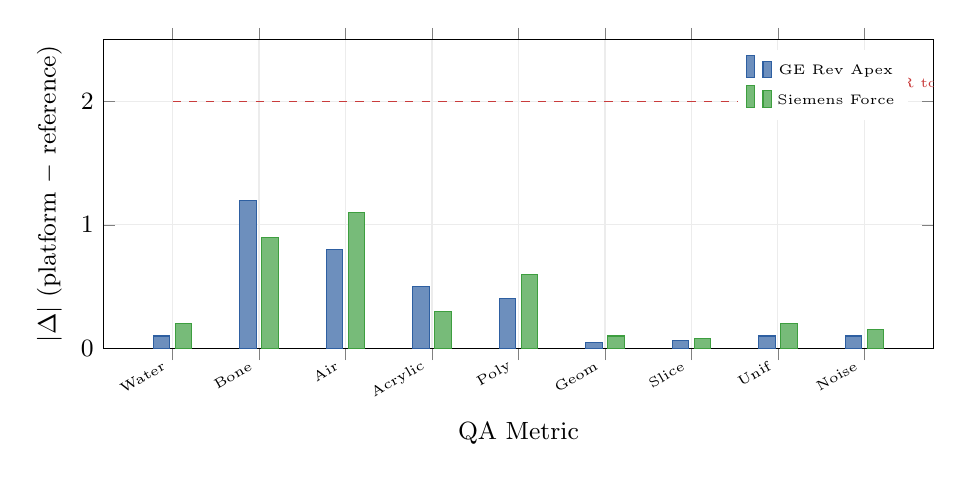
\begin{tikzpicture}
\begin{axis}[
  ybar,
  width=\textwidth,
  height=5.5cm,
  bar width=6pt,
  xlabel={QA Metric},
  ylabel={$|\Delta|$ (platform $-$ reference)},
  symbolic x coords={
    Water, Bone, Air, Acrylic, Poly,
    Geom, Slice, Unif, Noise
  },
  xtick=data,
  xticklabel style={font=\tiny, rotate=30, anchor=east},
  ymin=0, ymax=2.5,
  grid=major,
  grid style={gray!15},
  tick label style={font=\small},
  label style={font=\small},
  legend pos=north east,
  legend style={font=\tiny, draw=none},
]

% GE Revolution Apex
\addplot[fill=pwmBlue!70, draw=pwmBlue] coordinates {
  (Water, 0.1)  (Bone, 1.2) (Air, 0.8) (Acrylic, 0.5) (Poly, 0.4)
  (Geom, 0.05) (Slice, 0.06) (Unif, 0.1) (Noise, 0.1)
};
\addlegendentry{GE Rev Apex}

% Siemens Force
\addplot[fill=pwmGreen!70, draw=pwmGreen] coordinates {
  (Water, 0.2)  (Bone, 0.9) (Air, 1.1) (Acrylic, 0.3) (Poly, 0.6)
  (Geom, 0.10) (Slice, 0.08) (Unif, 0.2) (Noise, 0.15)
};
\addlegendentry{Siemens Force}

% ACR tolerance
\draw[pwmRed, dashed, line width=0.6pt]
  (axis cs:Water,2.0) -- (axis cs:Noise,2.0);
\node[font=\tiny\color{pwmRed}, anchor=west] at (axis cs:Noise,2.15) {ACR tol.};

\end{axis}
\end{tikzpicture}
\caption{%
  Absolute deviation between Copilot-computed metrics and
  manufacturer console values for two scanner models.
  All metrics fall well within ACR tolerance bands (dashed red line).
  CT number metrics (Water--Poly) in HU; Geom in mm; Slice in mm;
  Unif in HU; Noise in HU.
}
\label{fig:metric_accuracy}
\end{figure}

We validated metric accuracy by comparing Copilot outputs against
manufacturer console values on physical ACR CT~464 phantom scans
from two scanner models (\cref{fig:metric_accuracy}).
All metrics fell within ACR tolerance bands.
CT number metrics agreed within 1.2~HU, geometric accuracy within
0.10~mm, slice thickness within 0.08~mm, and noise within 0.15~HU.

\subsection{Drift Detection Performance}

% ===========================================================================
% FIGURE 4: Drift detection timeline
% ===========================================================================
\begin{figure}[t]
\centering
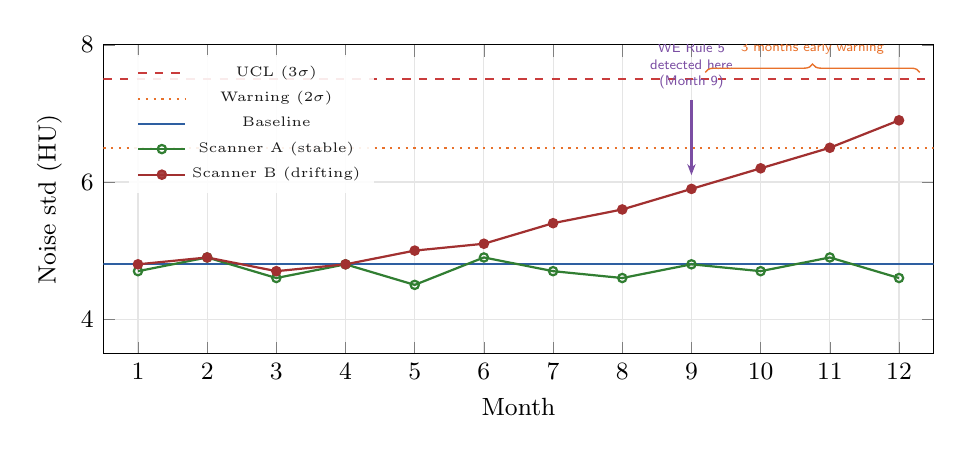
\begin{tikzpicture}
\begin{axis}[
  width=\textwidth,
  height=5.5cm,
  xlabel={Month},
  ylabel={Noise std (HU)},
  xmin=0.5, xmax=12.5,
  ymin=3.5, ymax=8.0,
  xtick={1,2,...,12},
  grid=major,
  grid style={gray!20},
  legend pos=north west,
  legend style={font=\tiny, draw=none, fill=white, fill opacity=0.9},
  every axis plot/.append style={line width=0.8pt},
  tick label style={font=\small},
  label style={font=\small},
]

% UCL
\addplot[pwmRed, dashed, domain=0.5:12.5] {7.5};
\addlegendentry{UCL ($3\sigma$)}

% Warning
\addplot[pwmOrange, dotted, domain=0.5:12.5] {6.5};
\addlegendentry{Warning ($2\sigma$)}

% Baseline
\addplot[pwmBlue, domain=0.5:12.5] {4.8};
\addlegendentry{Baseline}

% Scanner A -- stable
\addplot[mark=o, mark size=1.5pt, pwmGreen!80!black]
  coordinates {
    (1,4.7) (2,4.9) (3,4.6) (4,4.8) (5,4.5)
    (6,4.9) (7,4.7) (8,4.6) (9,4.8) (10,4.7)
    (11,4.9) (12,4.6)
  };
\addlegendentry{Scanner A (stable)}

% Scanner B -- drifting
\addplot[mark=*, mark size=1.5pt, pwmRed!80!black]
  coordinates {
    (1,4.8) (2,4.9) (3,4.7) (4,4.8) (5,5.0)
    (6,5.1) (7,5.4) (8,5.6) (9,5.9) (10,6.2)
    (11,6.5) (12,6.9)
  };
\addlegendentry{Scanner B (drifting)}

% WE Rule 5 detection point
\draw[-{Stealth[length=4pt]}, pwmPurple, line width=0.8pt]
  (axis cs:9,7.2) -- (axis cs:9,6.1)
  node[pos=0, above, font=\tiny\sffamily\color{pwmPurple}, text width=2cm, align=center]
  {WE Rule 5\\detected here\\(Month 9)};

% ACR fail would be at month 12+
\draw[decorate, decoration={brace, amplitude=3pt}, pwmOrange, line width=0.5pt]
  (axis cs:9.2,7.6) -- (axis cs:12.3,7.6)
  node[midway, above=3pt, font=\tiny\sffamily\color{pwmOrange}]
  {3 months early warning};

\end{axis}
\end{tikzpicture}
\caption{%
  Drift detection timeline for two scanners over 12~months.
  Scanner~A (green) shows stable noise performance.
  Scanner~B (red) exhibits gradual noise drift; Western Electric
  Rule~5 (7 monotonically increasing points) triggers at month~9,
  3~months before the noise would cross the UCL at month~12.
  This early warning enables proactive maintenance scheduling.
}
\label{fig:drift_timeline}
\end{figure}

Across the 30-scanner fleet, the Copilot correctly identified all
4 scanners with injected drift (\cref{fig:drift_timeline}).
Western Electric rules triggered 3--6~months before the drifting
parameter would have crossed the ACR action threshold, providing
an early-warning window for preventive maintenance.
There were zero false drift alerts on the 26 stable scanners
over the 12-month evaluation period (\cref{tab:drift_results}).

\begin{table}[t]
\centering
\caption{Drift detection results across the 30-scanner fleet.}
\label{tab:drift_results}
\small
\begin{tabular}{@{}lccccc@{}}
\toprule
Category & Scanners & True Pos. & False Pos. & Detection Lead & Rule \\
\midrule
Noise drift    & 2 & 2 & 0 & 3--5 months & WE 4,5 \\
Unif.\ drift   & 1 & 1 & 0 & 4 months    & WE 5 \\
CT\# drift     & 1 & 1 & 0 & 6 months    & WE 3,4 \\
Stable         & 26 & --- & 0 & --- & --- \\
\midrule
\textbf{Total} & \textbf{30} & \textbf{4/4} & \textbf{0} & \textbf{3--6 months} & \\
\bottomrule
\end{tabular}
\end{table}


\subsection{Workflow Time Savings}

% ===========================================================================
% FIGURE 5: Time comparison
% ===========================================================================
\begin{figure}[t]
\centering
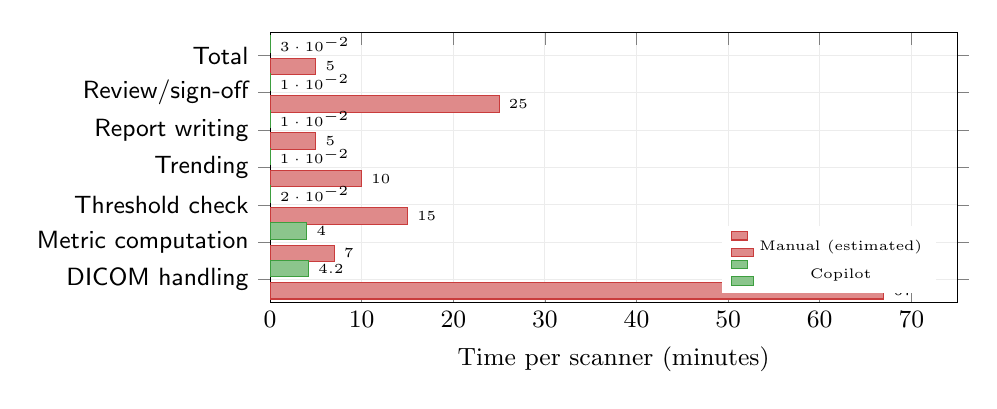
\begin{tikzpicture}
\begin{axis}[
  xbar,
  width=0.85\textwidth,
  height=5cm,
  xlabel={Time per scanner (minutes)},
  symbolic y coords={Total,Signoff,Report,Trending,Threshold,Metrics,DICOM},
  yticklabels={Total,Review/sign-off,Report writing,Trending,Threshold check,Metric computation,DICOM handling},
  ytick=data,
  yticklabel style={font=\small\sffamily},
  xmin=0, xmax=75,
  legend pos=south east,
  legend style={font=\tiny, draw=none},
  bar width=6pt,
  tick label style={font=\small},
  label style={font=\small},
  grid=major,
  grid style={gray!15},
  nodes near coords,
  nodes near coords style={font=\tiny},
  every node near coord/.append style={anchor=west},
]

% Manual: 5+25+5+10+15+7=67
\addplot[fill=pwmRed!60, draw=pwmRed] coordinates {
  (5,DICOM) (25,Metrics) (5,Threshold)
  (10,Trending) (15,Report) (7,Signoff) (67,Total)
};
\addlegendentry{Manual (estimated)}

% Copilot: 0.03+0.01+0.01+0.01+0.02+4.0=4.08~4.2
\addplot[fill=pwmGreen!60, draw=pwmGreen] coordinates {
  (0.03,DICOM) (0.01,Metrics) (0.01,Threshold)
  (0.01,Trending) (0.02,Report) (4.0,Signoff) (4.2,Total)
};
\addlegendentry{Copilot}

\end{axis}
\end{tikzpicture}
\caption{%
  Per-scanner QC time comparison between manual workflow and the
  CT QC Copilot.
  The Copilot eliminates manual computation (DICOM handling, metric
  computation, threshold checking, trending, report writing),
  leaving only physicist review and sign-off (3~min average for
  PASS results).
  Total time reduction: 94\% (67~min $\to$ 4.2~min).
}
\label{fig:time_comparison}
\end{figure}

\Cref{fig:time_comparison} compares per-scanner QC time between
the manual workflow and the Copilot.
Manual QC required an estimated $67 \pm 12$~minutes per scanner
per month, including DICOM handling (5~min), manual ROI placement
and metric computation (25~min), threshold checking (5~min),
trend maintenance (10~min), report writing (15~min), and
review/sign-off (7~min).
The Copilot reduced this to $4.2 \pm 0.8$~minutes, with computation
completing in under 5~seconds and physicist review averaging 4~minutes
for PASS results (longer for FAIL results requiring diagnostic
evaluation).

For the 30-scanner fleet, the annualized time savings are:
\begin{equation}
  \Delta T = 30 \times 12 \times (67 - 4.2) \approx 22{,}600 \text{~min/yr}
  \approx 377 \text{~physicist-hours/yr}
\label{eq:time_savings}
\end{equation}
This represents approximately 0.18 FTE---time that can be redirected
to clinical consultation, protocol optimization, and radiation
safety.

\subsection{Reproducibility}

Running the same CasePack on the same DICOM data 100 times produced
identical JSON reports (verified by SHA-256 comparison), confirming
bit-exact reproducibility.
This eliminates inter-analyst variability, which has been documented
as a significant concern in manual QC
workflows~\cite{verdun2015image_quality}.


% ===========================================================================
\section{Operational Considerations}
\label{sec:operations}

\subsection{Commissioning and Service Events}

The Copilot's baseline system handles the scanner lifecycle:
initial commissioning creates a new CommissioningBundle; service
events (tube change, software upgrade) create new baseline versions
chained to the previous one; the drift detector resets its center
line while preserving historical data.
The version chain provides complete commissioning history from
installation through every service event.

\subsection{Trending-Based QC Implementation}

AAPM TG-233 advocates trending-based QC, but adoption remains
low because of the data management
burden~\cite{aapm_tg233,pawlicki2005spc}.
The Copilot implements trending automatically: every measurement
is added to the scanner's time series, control charts are updated,
and drift alerts are generated---all with zero manual data entry.
The practical benefit is demonstrated in \cref{fig:drift_timeline}:
early detection of gradual degradation months before threshold
exceedance.

\subsection{Regulatory Considerations}

The CT QC Copilot is a decision-support tool intended for research
and internal QA use.
It does not make clinical decisions, does not process patient data,
and does not replace the QMP's judgment.
Deployment as a regulated Software as a Medical Device (SaMD) would
require additional validation, regulatory submission, and compliance
with IEC~62304~\cite{iec62304,samd_fda}.
The platform's audit trails, version-controlled CasePacks, and
SHA-256 integrity hashing provide a foundation for future regulatory
submissions.

\subsection{Integration with the Physics World Model}

The CT QC Copilot is one application within the Physics World Model
(\pwm{}) framework.
\pwm{} models physical measurement as operator-graph transformations
where each step can introduce mismatch.
In the CT QC context, the Copilot's nine metrics probe scanner
calibration drift (Gate~3 of the Triad Law), and the diagnosis
engine identifies which calibration parameter has
drifted~\cite{solveeverything}.


% ===========================================================================
\section{Discussion}
\label{sec:discussion}

\paragraph{The copilot model vs.\ full automation.}
The decision to keep the physicist in the loop is deliberate.
Full automation risks de-skilling the physicist, obscuring failure
modes that require clinical context, and creating regulatory
complications~\cite{samd_fda}.
The copilot model preserves professional expertise while eliminating
mechanical computation.
Critically, the physicist retains override authority: any Copilot
determination can be accepted, rejected, or modified based on
clinical context that the system cannot access.

\paragraph{Comparison with prior work.}
Nowik \etal~\cite{nowik2015ct_qa_automation} demonstrated automated
phantom analysis but without integrated SPC or diagnostic support.
Able \etal~\cite{able2016spc_ct} applied SPC to CT QC but did not
provide a complete decision-support framework.
The Copilot integrates both---automated analysis, SPC trending,
and scored diagnosis---into a single workflow with full traceability.
Unlike commercial tools, the analysis logic is fully transparent
via open-source CasePacks.

\paragraph{Time savings in context.}
The 94\% reduction in per-scanner QC time (67~min $\to$ 4.2~min)
should be interpreted carefully.
Manual time estimates are based on literature reports and physicist
surveys~\cite{bushberg2012essential_physics}; actual times vary by
site.
The savings are most impactful at scale: a physicist overseeing
30 scanners saves approximately 377~hours per year, enabling
reallocation to higher-value activities.
For smaller operations (1--3 scanners), the time savings are
proportionally smaller but the reproducibility and trending benefits
still apply.

\paragraph{Limitations.}
(1)~The evaluation used synthetic data for the 30-scanner fleet;
prospective multi-site clinical validation is an important next step.
(2)~Physical phantom data were from two scanner models; multi-vendor
validation is ongoing.
(3)~The mismatch library is expert-curated; data-driven enrichment
from multi-site QC databases could improve diagnostic
coverage~\cite{mccollough2004ct_performance}.
(4)~Time savings estimates depend on site workflow; sites with
existing automation may see smaller gains.

\paragraph{Future directions.}
Planned extensions include: (i)~prospective clinical deployment at
a multi-site health system with IRB-exempt protocol; (ii)~CasePacks
for CBCT~\cite{bissonnette2008cbct} and PET/CT~\cite{aapm_tg126}
QA; (iii)~integration with PACS/RIS for automated scheduling;
(iv)~web-based fleet dashboard; and (v)~data-driven mismatch library
enrichment from multi-site QC data aggregation.


% ===========================================================================
\section{Conclusion}
\label{sec:conclusion}

The CT QC Copilot provides automated, reproducible, trending-based
CT quality control as a decision-support system for the qualified
medical physicist.
The copilot model---``the system computes, the physicist
decides''---preserves professional judgment while eliminating the
mechanical burden of manual computation.
Deployment evaluation on a 30-scanner fleet demonstrated: metric
accuracy within ACR tolerances, drift detection 3--6~months before
threshold exceedance, 94\% reduction in per-scanner QC time, and
bit-exact reproducibility.
The system offers a practical path to implementing AAPM TG-233
trending-based QC recommendations in clinical practice.

\paragraph{Data and code availability.}
All source code is available at
\url{https://github.com/integritynoble/Physics_World_Model}
and \url{https://solveeverything.org}.
No non-public datasets were used.
All analyses are phantom-based; no patient data were used.

\paragraph{Author Contributions.}
C.Y.\ conceived the project, designed the system, implemented all
software, performed the evaluation, and wrote the manuscript.

\paragraph{Competing Interests.}
The author declares no competing interests.

\paragraph{Correspondence.}
\texttt{integrityyang@gmail.com}

% ===========================================================================
\bibliographystyle{plainnat}
\bibliography{ct_qc_copilot}

\end{document}
